\chapter{Training}
\label{ch:training}

\NS\ is pretrained on 25 trillion tokens in NVFP4 precision, extended to a
one-million-token context, fine-tuned on more than 7 million samples, trained
with reinforcement learning, and finally has its MTP heads retrained.

\section{NVFP4 Pretraining}

NVFP4~\cite{nvidia2025nvfp4} is a 4-bit format natively accelerated on NVIDIA
Blackwell GPUs. Each value is a 4-bit E2M1 number; blocks of 16 values share
an 8-bit (E4M3) scale, and a second FP32 scale is applied per tensor
(Figure~\ref{fig:nvfp4-format}), about 4.5 bits per value. Its smaller blocks
make it more accurate than MXFP4.

\begin{figure}[!htbp]
  \centering
  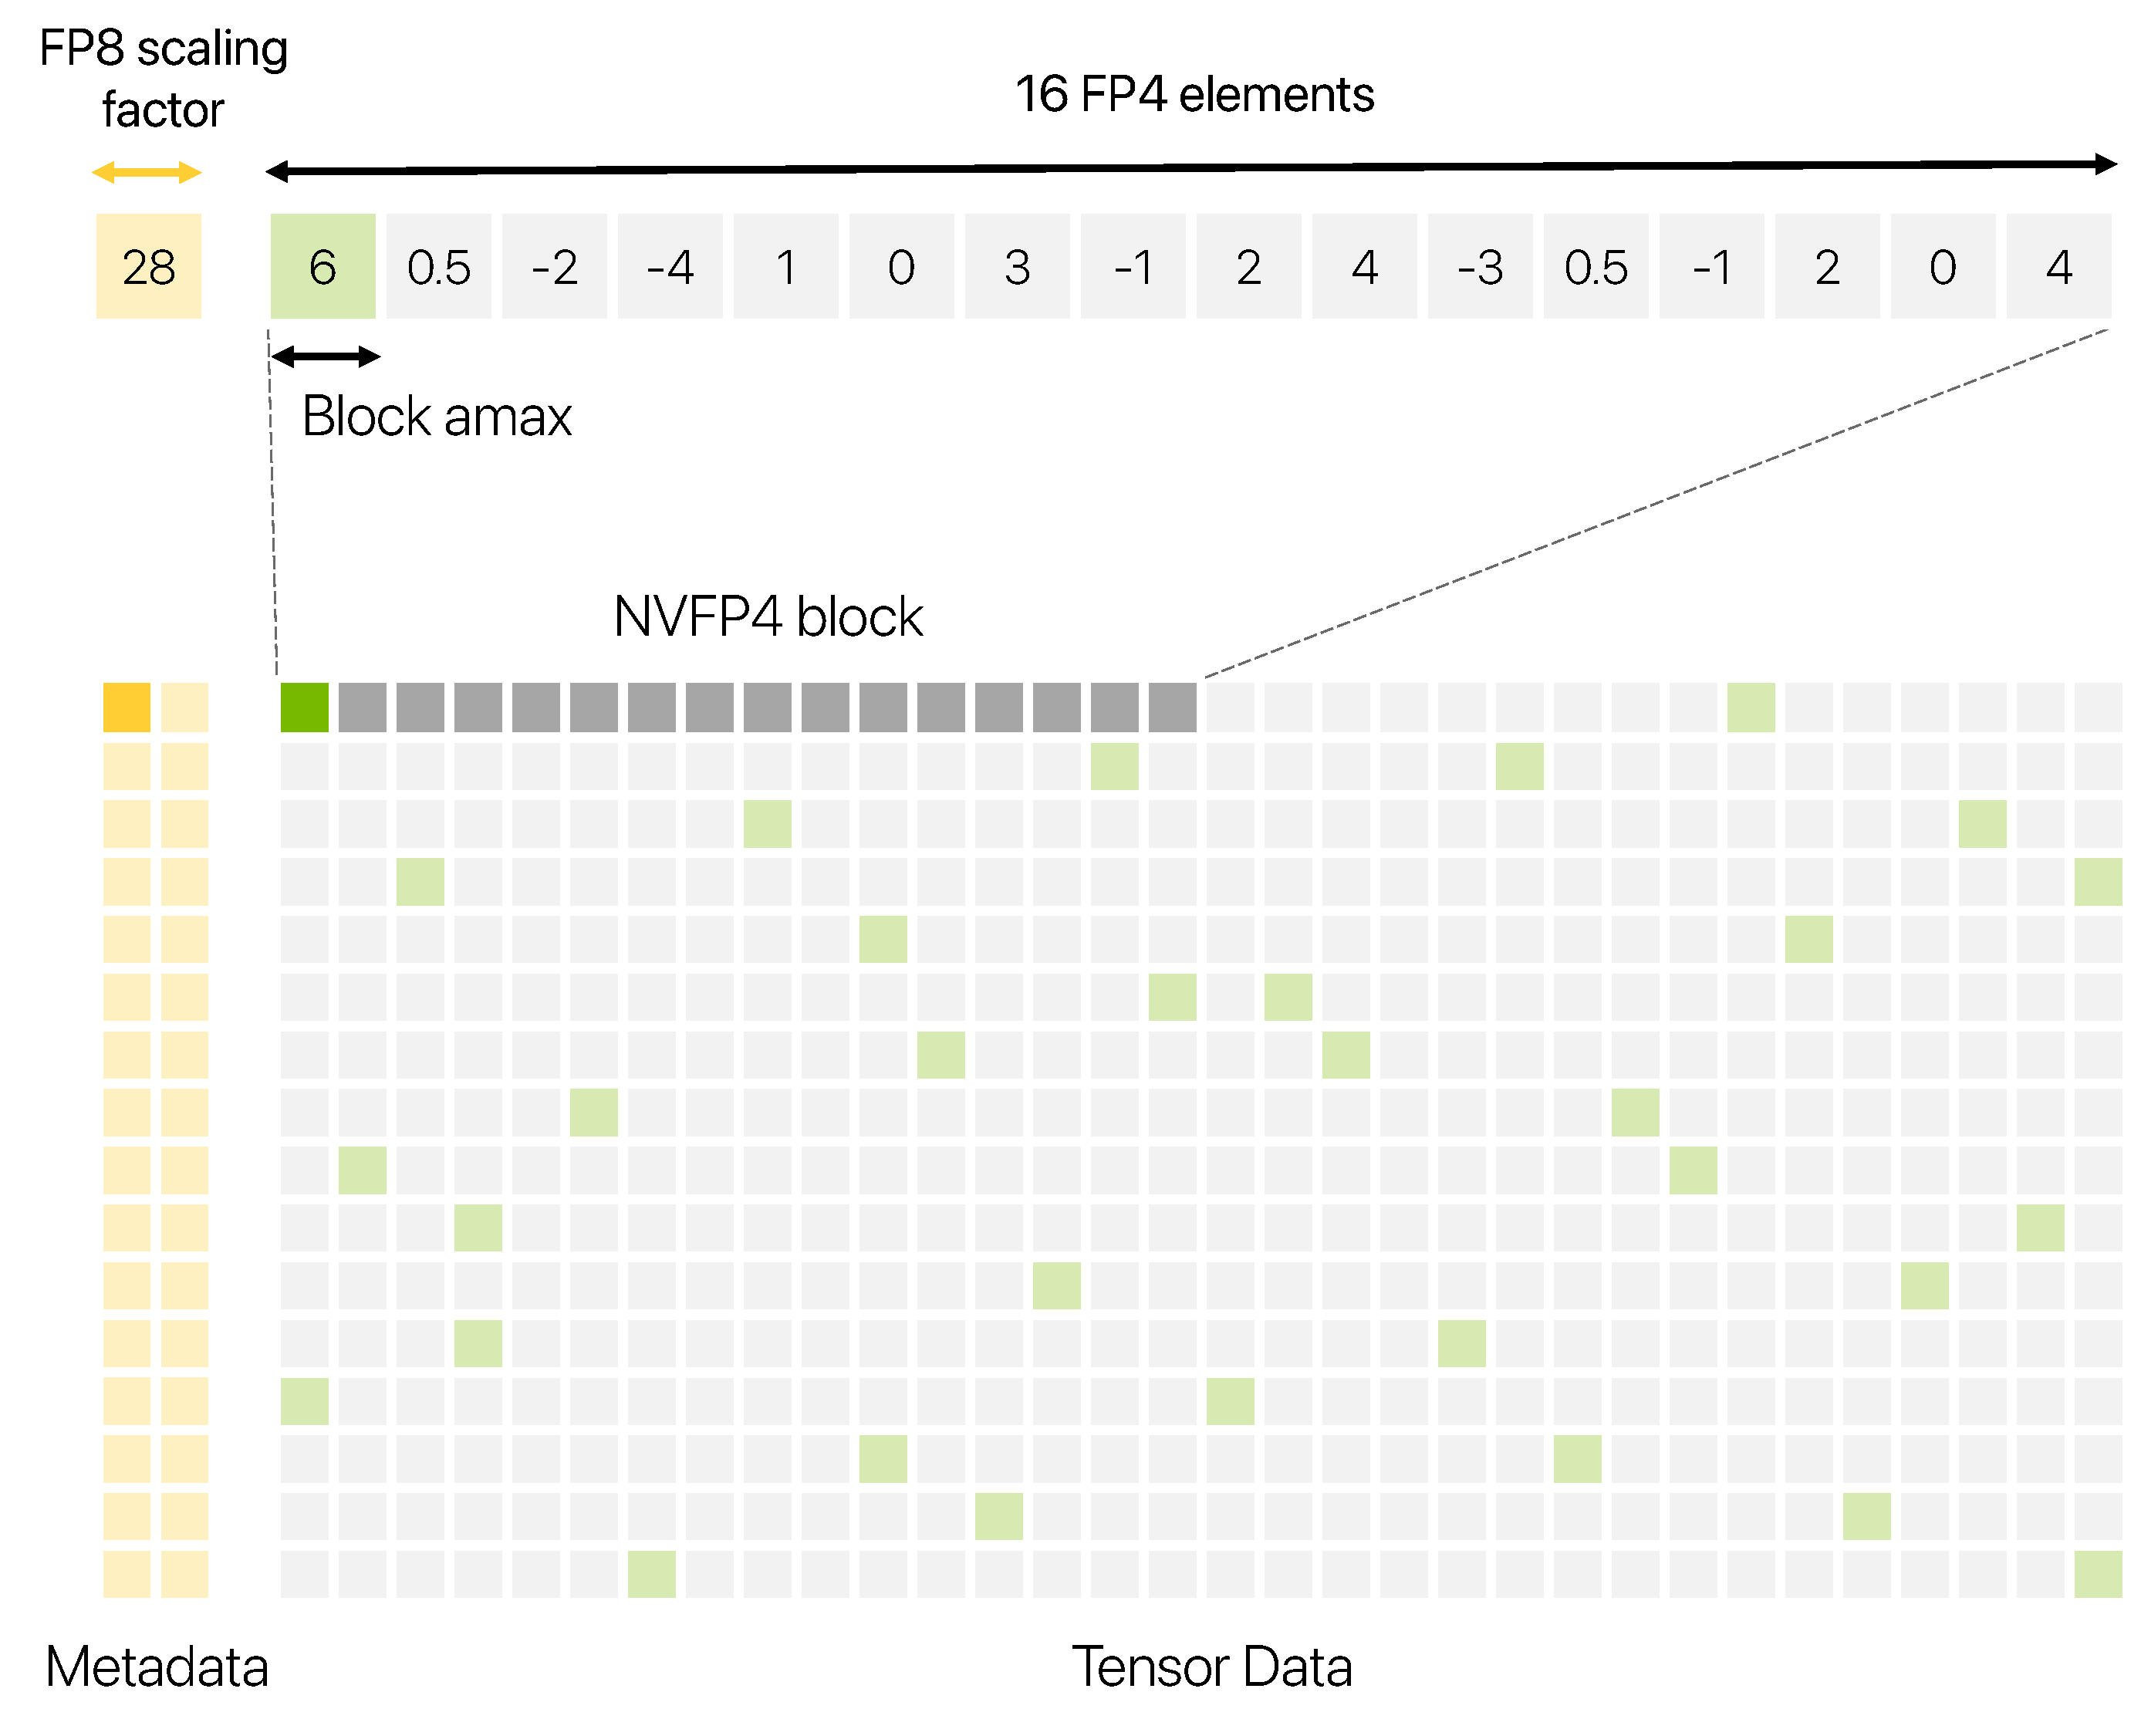
\includegraphics[width=0.48\linewidth]{nvfp4-fig01-format.pdf}
  \caption[A matrix stored in NVFP4 format]{A matrix stored in NVFP4: each
  block holds sixteen FP4 elements and one FP8 scale. \source{NVIDIA
  (2025)~\cite{nvidia2025nvfp4}, Fig.~1}}
  \label{fig:nvfp4-format}
\end{figure}

Simply rounding everything to 4 bits makes training diverge. The recipe uses
two-dimensional block scaling for weights, Random Hadamard Transforms to spread
outliers, stochastic rounding of gradients, and keeps a few sensitive layers in
higher precision (Table~\ref{tab:precision-train}). On a 12B model this kept
the loss close to FP8 over 10T tokens (Figure~\ref{fig:nvfp4-loss}).

\begin{figure}[!htbp]
  \centering
  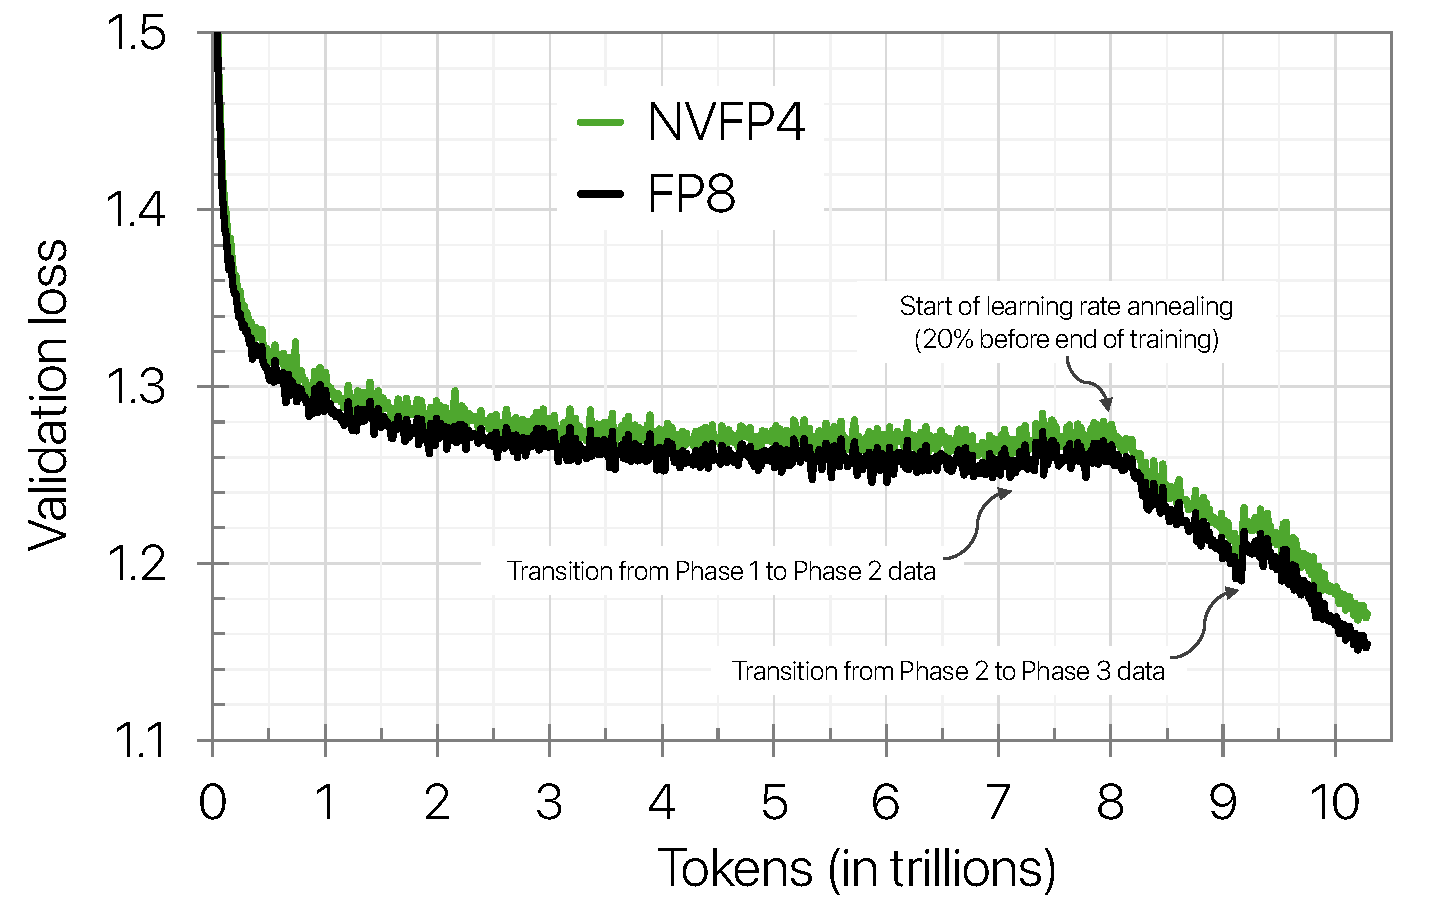
\includegraphics[width=0.6\linewidth]{nvfp4-fig02-val-loss.pdf}
  \caption[Validation loss of NVFP4 versus FP8 pretraining]{Validation loss of
  NVFP4 and FP8 pretraining for a 12B model. \source{NVIDIA
  (2025)~\cite{nvidia2025nvfp4}, Fig.~2}}
  \label{fig:nvfp4-loss}
\end{figure}

\begin{table}[!htbp]
\centering
\small
\caption[Training precision by layer type]{Training precision by layer type
(from~\cite{nvidia2026super}, Table~3)}
\label{tab:precision-train}
\begin{tabularx}{\linewidth}{@{}P{4.6cm}cL@{}}
\toprule
\textbf{Layer type} & \textbf{Format} & \textbf{Rationale} \\
\midrule
All linear layers unless noted & NVFP4 & Default \\
Final 15\% of the network & BF16 & Training stability at scale \\
Latent projections, embeddings & BF16 & Negligible effect on step time \\
MTP and attention layers & BF16 & Preserve fidelity of these few layers \\
Mamba output projection & MXFP8 & Avoids underflow seen with NVFP4 \\
\bottomrule
\end{tabularx}
\end{table}

Training was stable over all 25T tokens. Zero-valued weight gradients grew to
7\% of parameters; a controlled test on \NN\ showed NVFP4 produces about three
times more than BF16 because 4-bit quantization underflows tiny gradients
(Figure~\ref{fig:nvfp4-zeros}). Switching to MXFP8 at 19T tokens gave no
lasting downstream gain (Figure~\ref{fig:nvfp4-healing}), so NVFP4 was kept
throughout.

\begin{figure}[!htbp]
  \centering
  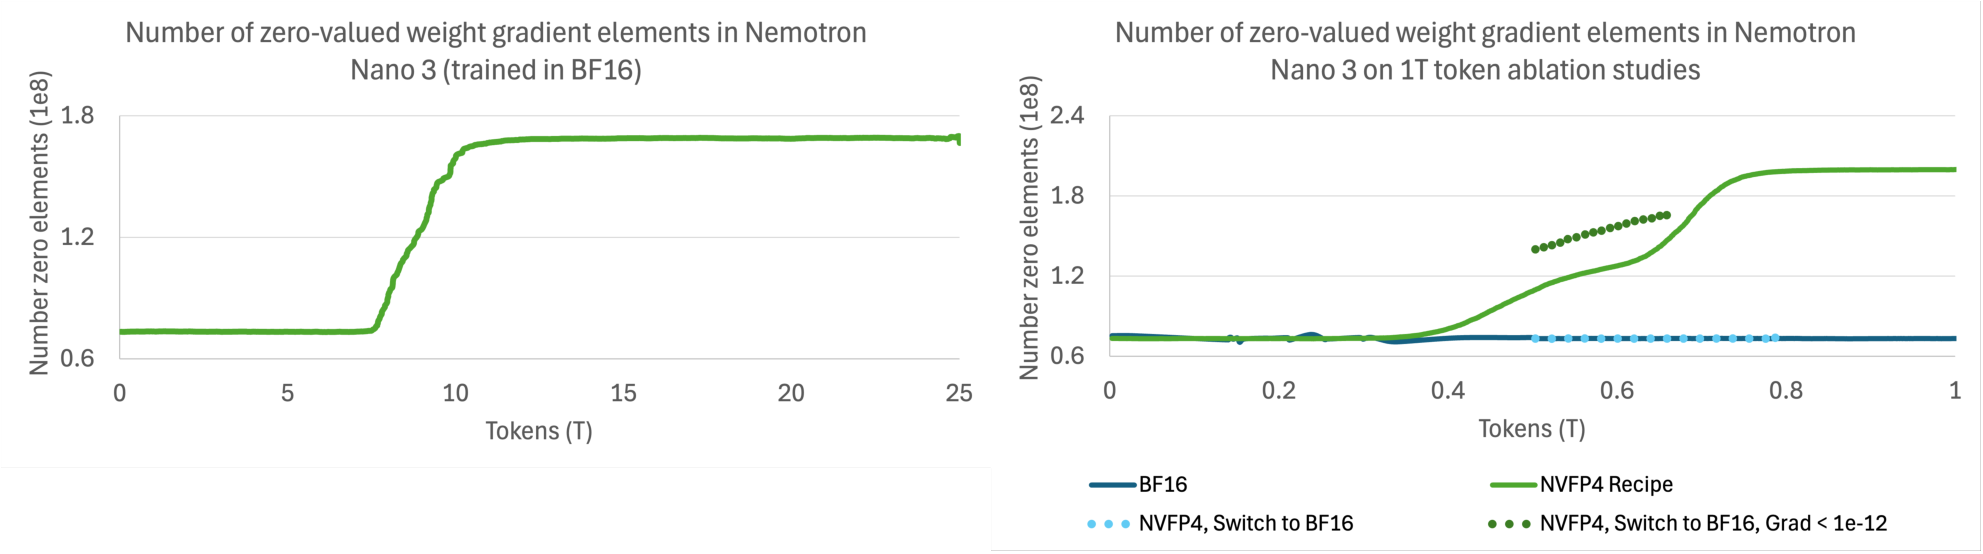
\includegraphics[width=0.92\linewidth]{n3s-fig07-nvfp4-zero-grads.pdf}
  \caption[Zero-valued weight gradients under NVFP4 and BF16 training]{Zero-valued
  weight-gradient elements on \NN\ under BF16 and NVFP4. \source{NVIDIA
  (2026)~\cite{nvidia2026super}, Fig.~7}}
  \label{fig:nvfp4-zeros}
\end{figure}

\begin{figure}[!htbp]
  \centering
  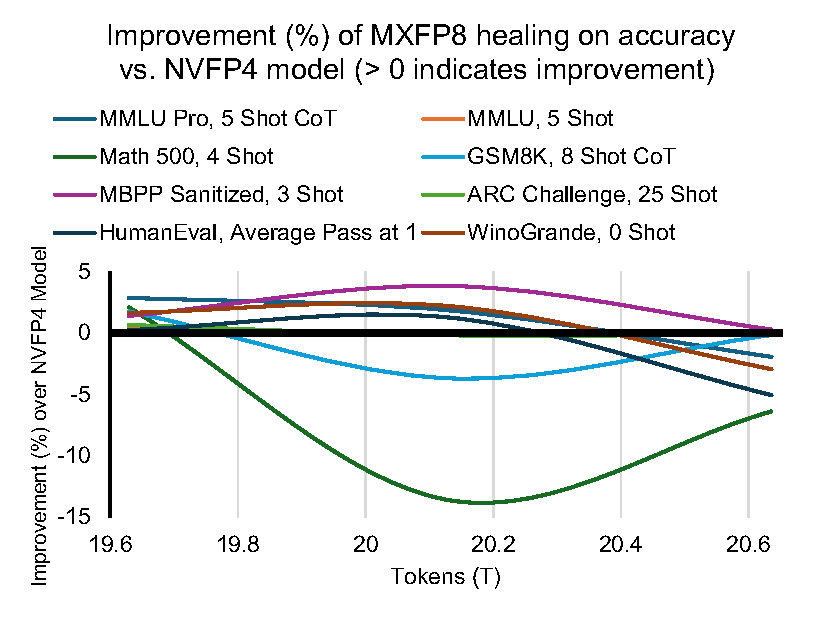
\includegraphics[width=0.52\linewidth]{n3s-fig09-nvfp4-healing.pdf}
  \caption[Effect of switching from NVFP4 to MXFP8 late in pretraining]{Change
  in downstream accuracy after switching to MXFP8. \source{NVIDIA
  (2026)~\cite{nvidia2026super}, Fig.~9}}
  \label{fig:nvfp4-healing}
\end{figure}

\section{Pretraining Data and Optimisation}

The corpus spans 16 categories---web crawl in quality tiers with synthetic
rewrites, mathematics, Wikipedia, code, academic, multilingual and synthetic
instruction data---plus new synthetic sets for code concepts, algorithmic
problems, economics, formal logic and multiple-choice reasoning. A two-phase
curriculum (Figure~\ref{fig:blends}) uses diverse data for the first 20T tokens
and shifts to high-quality sources for the last 5T.

\begin{figure}[!htbp]
  \centering
  \begin{subfigure}[b]{0.44\linewidth}
    \centering
    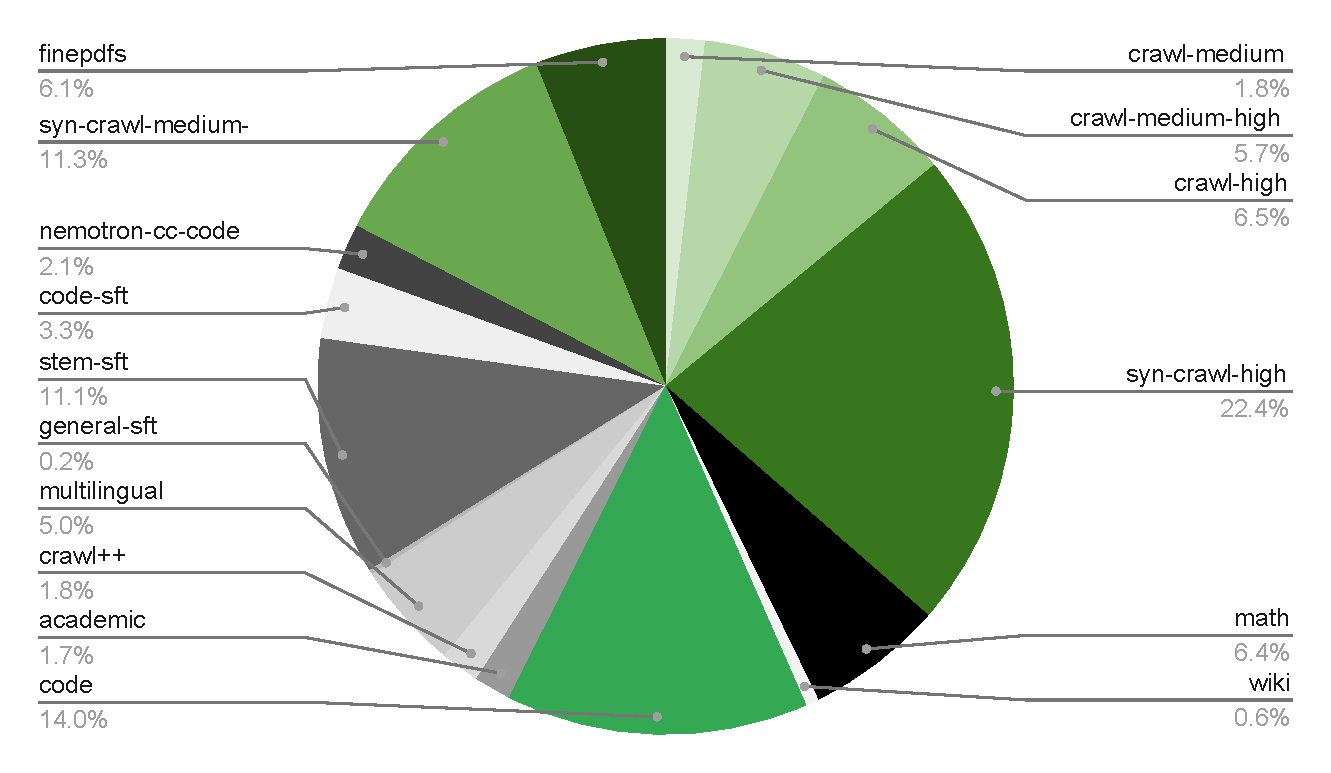
\includegraphics[width=\linewidth]{n3s-fig10a-phase1-blend.pdf}
    \caption{Phase 1}
  \end{subfigure}\hfill
  \begin{subfigure}[b]{0.44\linewidth}
    \centering
    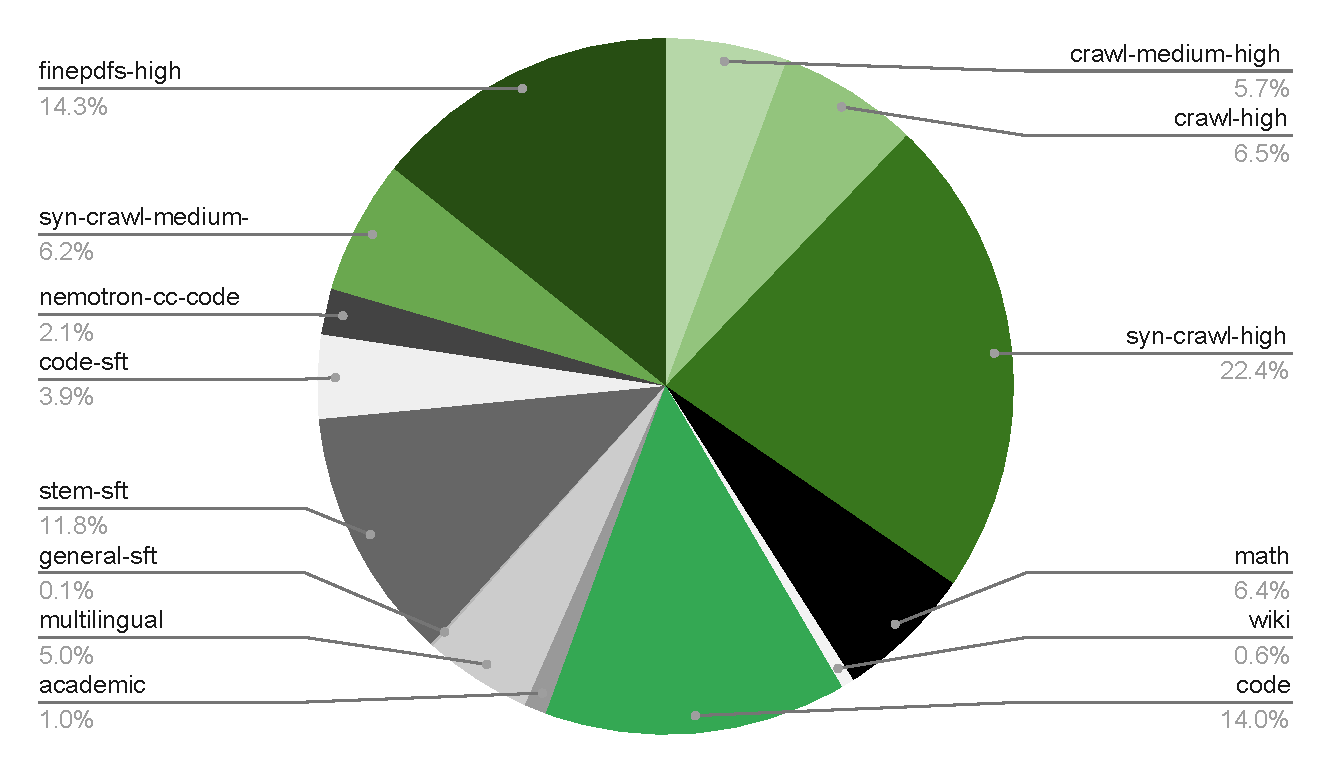
\includegraphics[width=\linewidth]{n3s-fig10b-phase2-blend.pdf}
    \caption{Phase 2}
  \end{subfigure}
  \caption[Data mixtures for the two pretraining phases]{Data mixtures for the
  two pretraining phases. \source{NVIDIA (2026)~\cite{nvidia2026super},
  Fig.~10}}
  \label{fig:blends}
\end{figure}

Training uses AdamW with a Warmup--Stable--Decay schedule (peak learning rate
$4.5 \times 10^{-4}$), 8192-token sequences and about 25M tokens per step.
Instead of separate decay runs to track progress, recent checkpoints were
\emph{merged} by weighted averaging; merges scored 2--4 points higher than raw
checkpoints during the stable phase (Figure~\ref{fig:merge}), saving an
estimated 16\% of pretraining compute.

\begin{figure}[!htbp]
  \centering
  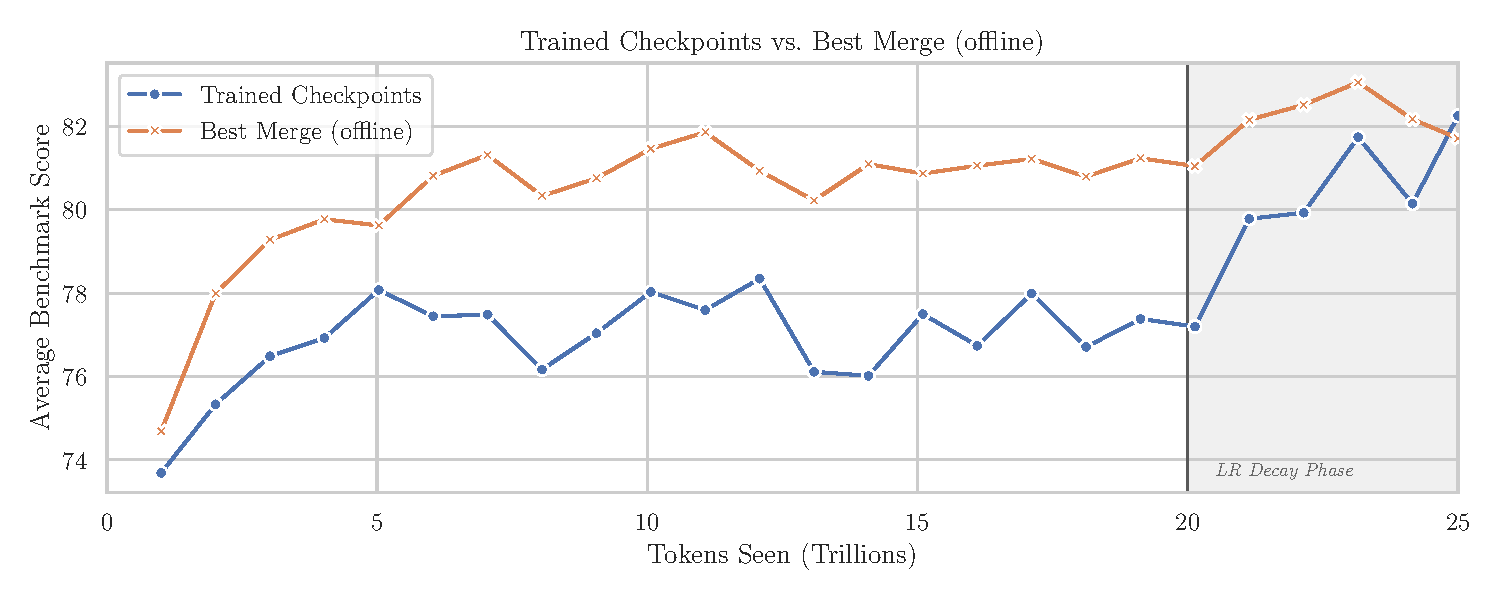
\includegraphics[width=0.85\linewidth]{n3s-fig11-checkpoint-merge.pdf}
  \caption[Trained checkpoints versus merged checkpoints during pretraining]{Average
  accuracy over 12 benchmarks for trained and merged checkpoints.
  \source{NVIDIA (2026)~\cite{nvidia2026super}, Fig.~11}}
  \label{fig:merge}
\end{figure}

A final long-context phase continues at a constant learning rate on 20\%
long-document question-answering data and 80\% Phase~2 data: 34B tokens at a
context of 1,048,576 tokens, then 17B tokens alternating 1M and 4k sequences to
remove a small regression on mathematics. Million-token sequences need 64-way
context parallelism and 64-way expert parallelism on GB200 GPUs; this is
practical because 80 of the 88 layers have no quadratic cost.

\section{Supervised Fine-Tuning}

Post-training follows Figure~\ref{fig:posttraining}. SFT uses more than 7
million samples. A single-stage SFT degraded tasks with long inputs and short
outputs, so two stages with different loss normalisation are used. For a batch
$\mathcal{B}$ of conversations $c$, with output positions $\mathcal{O}_c$ and
token loss $\ell_t$, Stage~1 averages over all output tokens and Stage~2 first
within each conversation:
\begin{equation}
  \mathcal{L}_{\text{tok}} =
  \frac{\sum_{c \in \mathcal{B}} \sum_{t \in \mathcal{O}_c} \ell_t}
       {\sum_{c \in \mathcal{B}} |\mathcal{O}_c|},
  \qquad
  \mathcal{L}_{\text{samp}} =
  \frac{1}{|\mathcal{B}|} \sum_{c \in \mathcal{B}}
  \frac{1}{|\mathcal{O}_c|} \sum_{t \in \mathcal{O}_c} \ell_t .
\end{equation}
Stage~1 gives strong token-level supervision that induces reasoning; Stage~2
stops very long outputs from dominating, restoring long-input, short-output
behaviour. Stage~1 packs sequences up to 256k tokens and Stage~2 up to 512k.
Agentic data---GitHub issues, terminal use, web search, SQL, tool calling and
more---takes a much larger share than for \NN\ (Figure~\ref{fig:sft-blend}).
The model supports reasoning off, regular and a new low-effort mode.

\begin{figure}[!htbp]
  \centering
  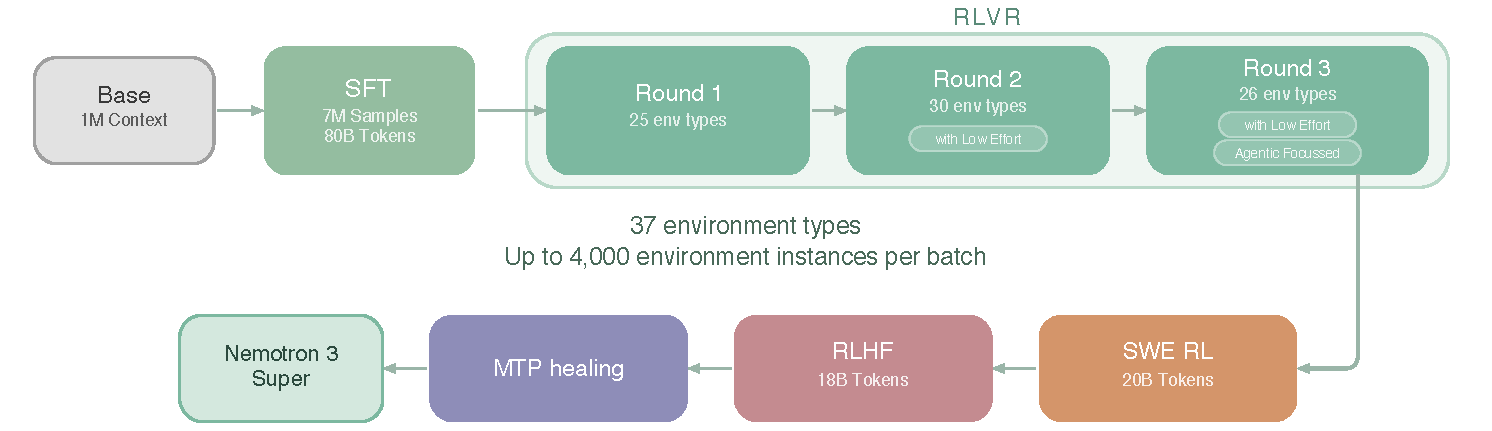
\includegraphics[width=0.92\linewidth]{n3s-fig12-posttraining-stages.pdf}
  \caption[Post-training pipeline of Nemotron 3 Super]{Post-training pipeline:
  SFT, three RL stages and MTP healing. \source{NVIDIA
  (2026)~\cite{nvidia2026super}, Fig.~12}}
  \label{fig:posttraining}
\end{figure}

\begin{figure}[!htbp]
  \centering
  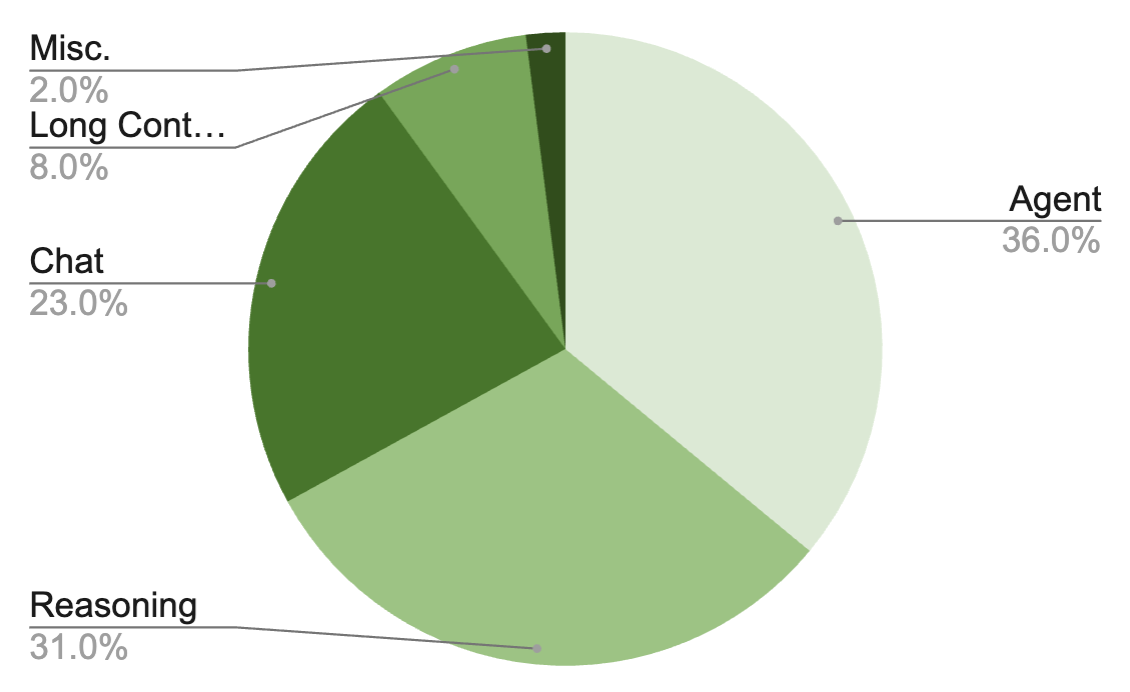
\includegraphics[width=0.52\linewidth]{n3s-fig16-sft-blend.jpg}
  \caption[SFT data blend for Nemotron 3 Super]{SFT data blend for \NS.
  \source{NVIDIA (2026)~\cite{nvidia2026super}, Fig.~16}}
  \label{fig:sft-blend}
\end{figure}

\section{Reinforcement Learning}

\textbf{Stage 1 -- RL from verifiable rewards.} The model is trained jointly
on 21 environments and 37 datasets (mathematics, code, STEM, safety, chat,
long context, agentic tasks) where rewards can be checked automatically.
Training on all at once avoided the regressions seen with single environments.
Easy prompts are filtered and the rest ordered by difficulty, a curriculum
shown to help on \NN\ (Figure~\ref{fig:rl-curriculum}). The algorithm is
asynchronous GRPO: inference workers generate trajectories continuously into a
buffer, full batches go to the trainer, and updated weights are pushed back
with workers never more than one step behind. Each step uses 256 prompts with
16 responses each, with generation length raised from 49K to 64K tokens. For
long-horizon agentic tasks, \emph{PivotRL} reuses expert trajectories and
focuses training on the ``pivot'' turns where the model is uncertain.

\begin{figure}[!htbp]
  \centering
  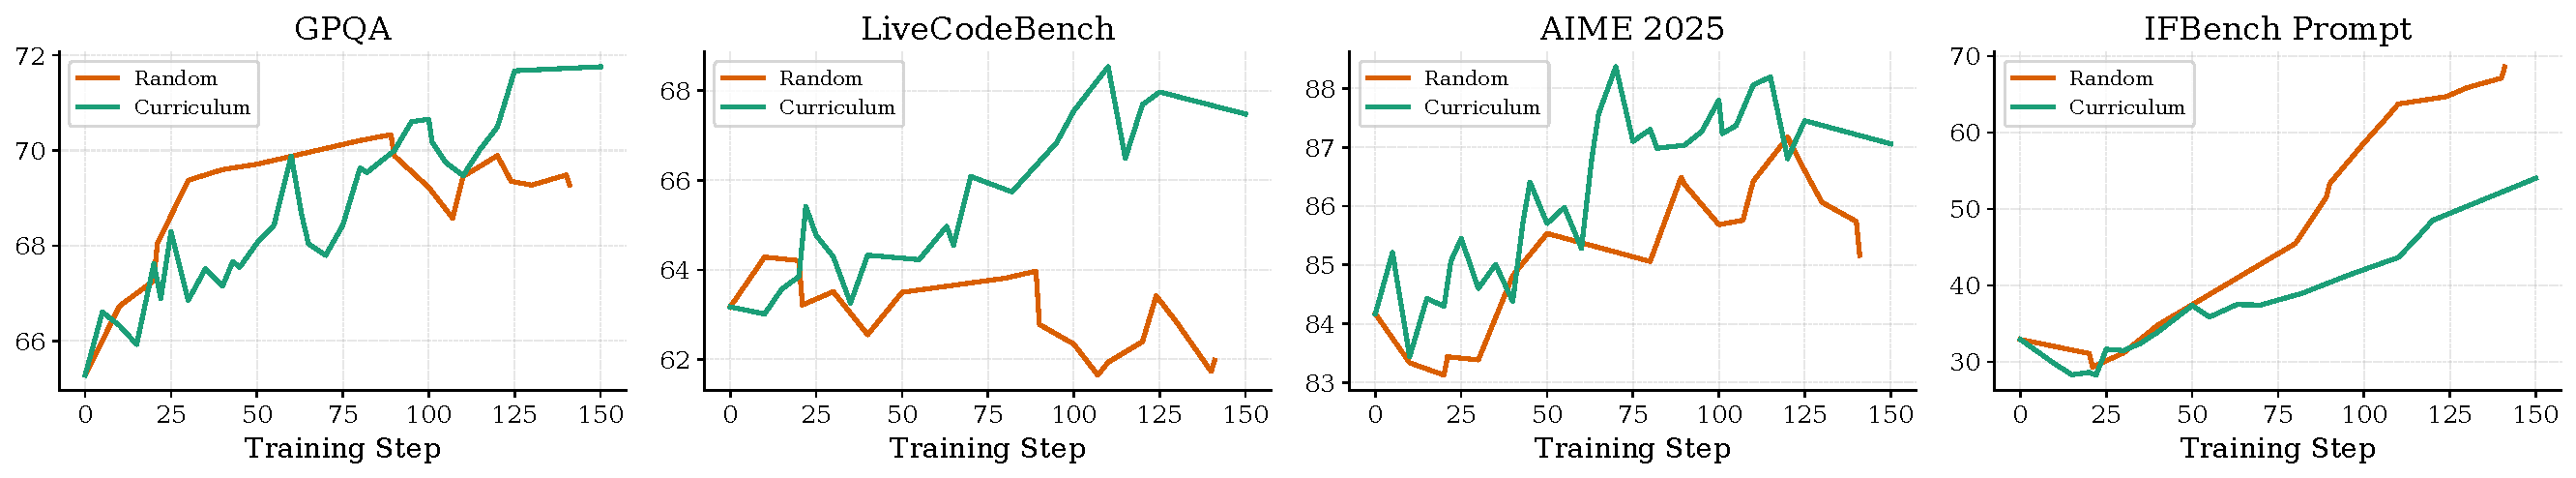
\includegraphics[width=0.85\linewidth]{nano3-fig07-rl-curriculum.pdf}
  \caption[Curriculum sampling versus random sampling in RL]{Curriculum versus
  random sampling during RL on \NN. \source{NVIDIA
  (2025)~\cite{nvidia2025nano3}, Fig.~7}}
  \label{fig:rl-curriculum}
\end{figure}

\textbf{Stage 2 -- Software engineering.} Each rollout runs an agent in a
container to produce a code patch, rewarded by the repository's tests.

\textbf{Stage 3 -- RL from human feedback.} A generative reward model trained
on human preferences improves instruction following and interaction quality.

\textbf{MTP healing.} Finally the network is frozen and only the MTP heads are
retrained on the model's own outputs, restoring their drafting accuracy.
